\graphicspath{{Articles-bons-a-composer/01_Spitz-Oener/01_graphs}}

% ATTENTION: bibliographie manquante dans cet article, la demander à l'auteure

% L'article tel que livré : ortho-typo et édition (TODO)

\begin{Article}[Titre={Regime Change and Occupational Mobility: Former GDR Workers During the ``Wende''},
Auteur=Alexandra Spitz-Oener\thanks{Humboldt-Universit\"at zu Berlin, RFBerlin and Institute for Employment Research (IAB)}]

\label{SpitzOener}
\selectlanguage{english}

    \begin{refsection}[Spitz]
        
% {\large\bf Regime Change and Occupational Mobility:\\ Former GDR Workers During the ``Wende''}

% {\large\bf Alexandra Spitz-Oener}\\


\begin{resume}
Using novel data linking administrative labor market information of German Democratic Republic (GDR) workers before and after reunification, I investigate occupational mobility during the ``Wende'' (1989-1992). I compare GDR workers' patterns with Federal Republic of Germany (FRG) workers from the same birth cohort. The results indicate diverse occupational mobility facets, including upgrading and downgrading. Notably, GDR workers exhibited much higher occupational mobility dynamics than the corresponding FRG cohorts. Regarding transitions to non-employment, the oldest cohort (aged 58-60 in 1989) drives the aggregate figures in both parts of Germany, reflecting the widespread application of early retirement schemes at the time.
\end{resume}

\remerciementsEng{This article highlights one aspect of the keynote lecture given by Alexandra Spitz-Oener at the 39th Journées de Microéconomie Appliquée on June 8rd, 2023. Spitz-Oener gratefully acknowledges financial support from the German Sciences Foundation (DFG) through the CRC-TRR 190, Project No. 280092119. The project played a pivotal role in co-funding the construction of the data used in this study. The data was created jointly with the Research Data Center (FDZ) of the Federal Employment Agency at the Institute for Employment Research (IAB). Special thanks are owed to Dana M\"uller and the dedicated team at the FDZ involved at various stages for the excellent collaboration, particularly Manfred Antoni, Matthias Umkehrer, and Florian Zimmermann. The data construction process is documented in the FDZ method report \textcite{LiepmannMuller2018}.
    More information, including information on data access, can be found here: 
    \url{https://doi.org/10.5164/IAB.FDZD.2213.de.v1}}
    
    %\href{https://fdz.iab.de/en/pd_hd/data-fund-of-societal-work-power-linked-with-administrative-data-of-the-institute-for-employment-research-iab-gav-adiab-1975-2019/}{IAB-FDZ}.

    
%===========================================================%
\section{Introduction}
On June 30, 1990, at midnight, the German Economic, Monetary, and Social Union was formally realized. It involved the integration of the former German Democratic Republic (GDR) into the Federal Republic of Germany (FRG). It represented a complete change of regime for the GDR, which brought about several key changes: the replacement of the East German mark with the Deutsche mark, the removal of trade barriers, the harmonization of the legal, tax, and social insurance systems, and the elimination of all existing obstacles to the movement of capital and labor. Shortly thereafter, a noticeable price-cost squeeze emerged, rendering East German manufacturers incapable of selling their products at prices that allowed them to operate profitably. The challenge extended beyond finding new buyers in West Germany or other countries; they also experienced a decline in demand from their East German domestic base, who redirected their spending towards Western products. This had a tremendous effect on the labor market in East Germany. From 1989 to 1992, employment declined by 35 percent, and unemployment rose from officially zero to more than 15 percent.\footnote{The characterization of the historical events and the figures presented in this paragraph are taken from \textcite{AkerlofRoseYellenHessenius1991}, and \textcite{BurdaHunt2001}.}

The macroeconomic facts of the immediate effects of the system transition are by now well documented. However, evidence on the individual consequences is quite scarce because comprehensive individual-level data of GDR people from both GDR times and after the Berlin Wall came down was missing. In this paper, I document the extent of occupational mobility for GDR workers between 1989 and 1992 using novel individual-level administrative data. The data in 1989 describes the occupational structure of GDR workers in the system of departure (the GDR), and the latter year describes the same GDR workers shortly after reunification, i.e. in the system of destination. In the past, research on German reunification with individual-level administrative data has faced two challenges: Firstly, the data suffered from a notable absence of information concerning GDR workers during the GDR era. Having comprehensive data on individuals in both the economy of origin and the destination is of paramount importance, especially when examining the individual consequences of a systemic transition. Secondly, in most data sets, identifying GDR workers is complicated even after reunification -- when, for example, the German administrative data covered East Germany -- as East Germans have German nationality and cannot be distinguished from Germans of West German origin in data sets that rely on nationality to identify the different demographic groups.


In this paper, I follow a cohort approach when investigating occupational mobility between 1989 and 1992 and compare GDR workers of a specific cohort with FRG workers of the same cohort. First, different birth cohorts were subject to different political, economic, and educational regimes at different ages when growing up. Secondly, when observing occupational mobility between 1989 and 1992, the results might depend on the age of individuals. Following a cohort approach and comparing GDR and FRG workers who were the same age in 1989 allows me to net out the age effects in the results.

The analyses reveal interesting differences in the education and occupational structure of GDR and FRG workers in 1989. First, the share of skilled and unskilled occupations was higher among GDR workers than FRG workers, at the expense of employment in professional and semi-professional occupations. There are also important gender differences, with GDR female workers being more educated than FRG female workers; however, the latter does not translate to a similar extent into more employment of female GDR workers in professional and semi-professional occupations than in the FRG. In addition, the employment share of female GDR workers in skilled occupations is considerably smaller than it is for FRG female workers.    

The results also suggest that comparing GDR and FRG workers' labor market developments between 1989 and 1992 is potentially very important, as is following a cohort approach. In addition, the detailed occupational mobility patterns are heterogeneous, involving more pronounced upward and downward occupational mobility of GDR workers of a cohort compared to FRG workers of the same cohort, together with FRG workers being much more occupational immobile than GDR workers. When it comes to transitions into non-employment, the largest difference is observed for the oldest cohort of men, those born between 1929-1931. This reflects the vast application of the early-retirement schemes that Germany then used, which applied to workers older than 55 in both East and West Germany (see \textcite{BorschSupranSchmidt2001}, among others). For women of this oldest cohort, it was those in the FRG who experienced transitions to non-employment to an even larger extent than GDR women. This was clearly not the case for women of the other birth cohorts, for which transitions into non-employment were much higher for GDR women than FRG women.


The data set used in this study is well-suited to complement existing work on German reunification. Earlier studies on the labor market trajectories of East Germans after reunification used, for example, the BASiD data \parencite{EmmlerFitzenberger2020}, Microcensus \parencite{FuchsSchundelnSchundeln2009}, Qualification and Career Survey \parencite{PrantlSpitzOener2020,PrantlSpitzOener2009}, aggregated unemployment or migration data \parencite{FuchsSchundelnIzem2012}, the GSOEP \parencite{BurdaHunt2001,Hunt2006,AlesinaFuchsSchundeln2007,FuchsSchundelnSchundeln2009,FuchsSchundelnIzem2012,Stauder2018,EmmlerFitzenberger2020}, or the East German Life History Survey \parencite{HuininkSolga1994}.

The study is structured as follows: the next section discusses the historical background. Section \ref{data} introduces the data and defines the main variables. In Section \ref{StatusQuo}, I characterize the GDR and FRG workers in 1989, and in Section \ref{1989to1992}, I show the results on occupational mobility between 1989 and 1992. Section \ref{Concl} concludes.

%===============================================================================%
\section{Regime Change and the Labor Market}


Because the GDR political and economic system was integrated into the FRG system very rapidly after 1989, it is hard to imagine another example of regime change at a faster pace. When it comes to the labor market, it is important to realize that the GDR labor market was organized fundamentally differently than the West German or any other Western-style labor market. In fact, in the planned economy of the GDR, there was no labor market (\textcite{Hoene1991}; \textcite{LutzNickelSchmidtSorge1996}): the workforce and individual careers were allocated and decided upon according to the economic plan (\textcite{Gruenert1996}, among others). 

One of the factors that are discussed when it comes to the potential reasons for the failure of the GDR system is the absence of structural changes. Looking at the industry structure of employment in the GDR, it becomes clear that the sectoral structure of employment was stable in the GDR for many decades. Figure \ref{Fig1a} shows no signs of structural changes between 1975 to 1989. The figure also illustrates that this changed dramatically after 1989. In less than three years, employment in manufacturing declined from more than 3.3 million to less than 1.5 million, making it the sector that was hit the strongest in terms of employment by the reunification shock. Agriculture, forestry, and fishing were also subject to large employment declines, from about 1.5 million in 1989 to about 250 thousand in 1992. Services were the only sector that expanded employment considerably during this time, and construction also saw its employment increase, even though much less than the services sector.

In comparison, structural changes evolved smoothly in West Germany (Figure \ref{Fig1b}). Up to 1989, employment in the services sector increased from about 3.5 million to about 5 million, whereas employment in manufacturing fluctuated around 8 million. Only after 1991/1992 the steady increase in employment in the service sector slowed down, and employment in manufacturing declined considerably.

%====================================================================%
\begin{figure}
\caption{\textbf Sectoral Employment in East and West Germany, 1975--1998}\label{fig1}
     \centering
     \begin{subfigure}[b]{0.8\textwidth}
         \centering
         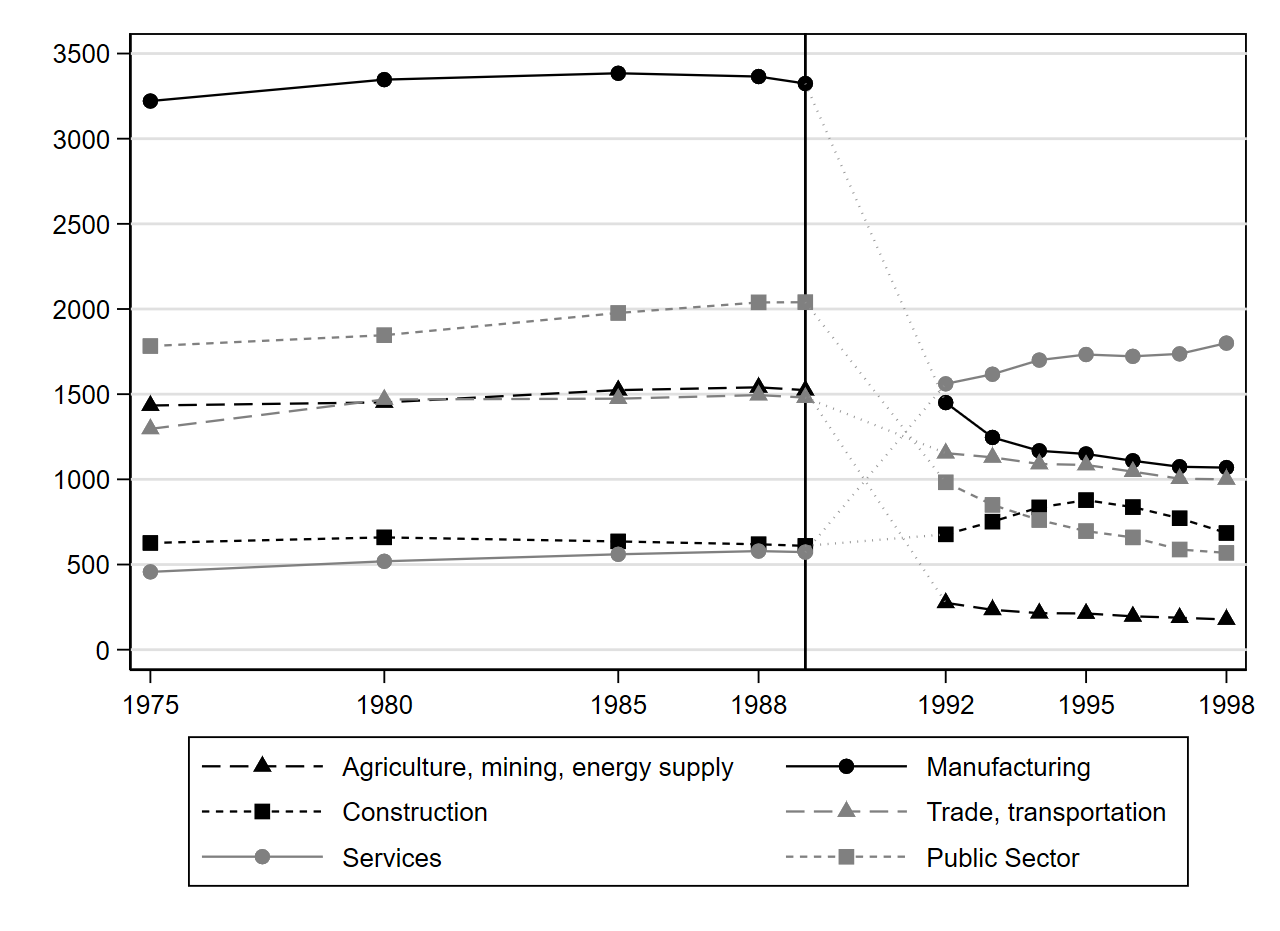
\includegraphics[width=\textwidth]{emp_East.png}
         \caption{East}
         \label{Fig1a}
     \end{subfigure}
     \hfill
     \begin{subfigure}[b]{0.8\textwidth}
         \centering
         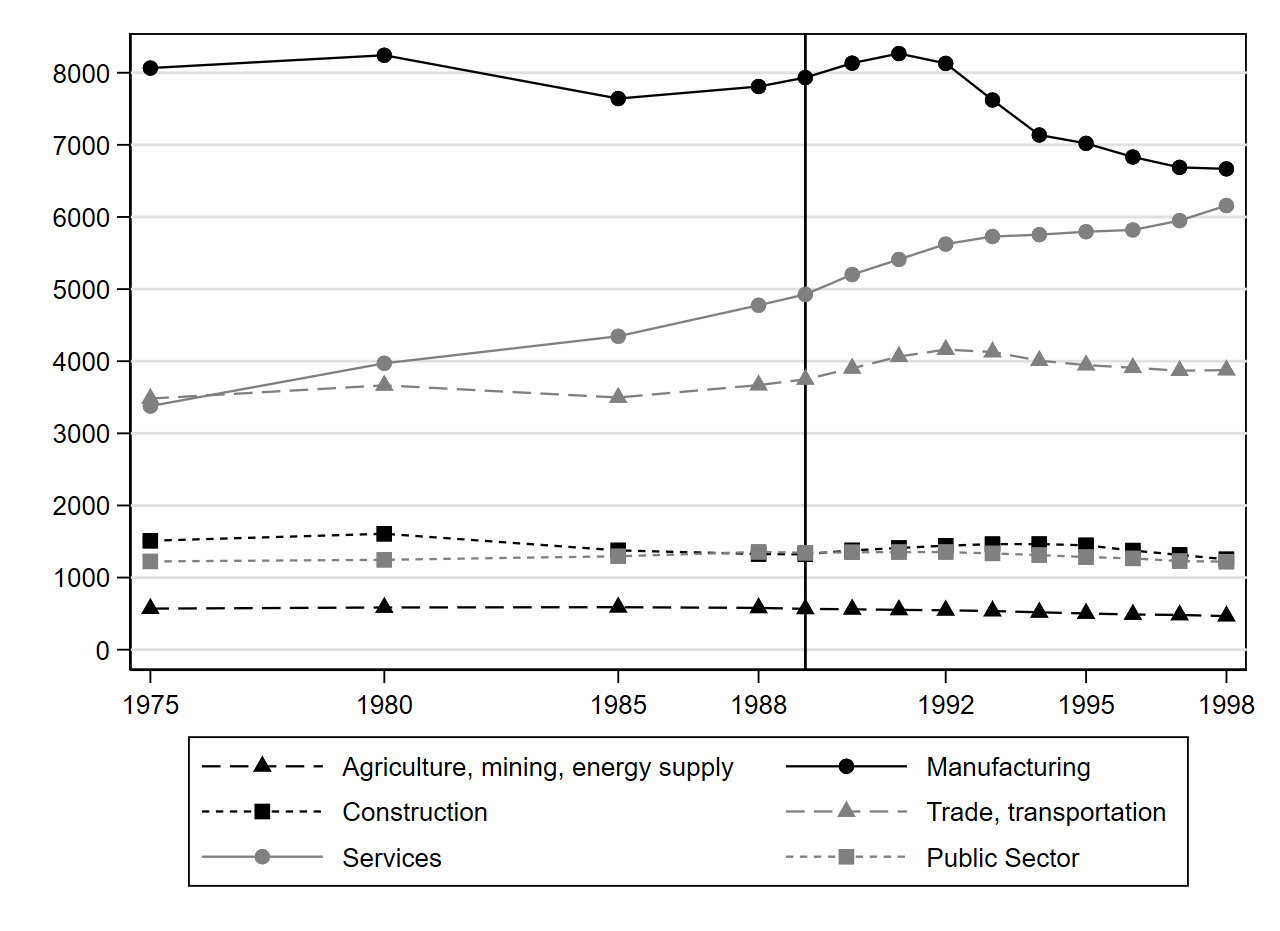
\includegraphics[width=\textwidth]{emp_West.png}
         \caption{West}
         \label{Fig1b}
     \end{subfigure}
     {\footnotesize
    \hspace*{0.1cm}\parbox[h]{\linewidth}{Notes: Y-scale in thousands of workers. The figure corresponds to \cite{FindeisenLeePorzioDauth2021}, Figure~2. The authors generously made the data available for replication. They provide details on the data sources.}}
\end{figure}
%\newpage
%=====================================================================%

The change in paradigm for the East German labor market is also visible in the evolution of unemployment. Unemployment did not officially exist in the GDR, with the right to work being part of the constitution.  Figure \ref{fig2} shows that this changed rapidly after the Wall fell. In 1991, the first year it was officially recorded for East Germany, the unemployment rate among East German men was 8.7\%. With 11.9\%, it was even higher among East German women. It gradually increased for East German men, first relatively slowly, but it accelerated after 1995 and reached 17.5\% in 1998. For East German women, the increase in the unemployment rate was faster during the first half of the 1990s and then remained relatively stable at around 20\%. Throughout the observation period, the unemployment rate among East German women was larger than among East German men.

The change in the unemployment rate in West Germany was much smoother during this period, albeit not constant. In 1988, with 9.4\%, West German women also experienced a relatively high level of unemployment, which declined to 7.0\% in 1991 before increasing even beyond the initial level to 10.2\% in 1998. West German men experienced an unemployment rate of 6.5\% in 1988, which declined to 5.0\% in 1990 before catching up to (and in some years even overtaking) the unemployment rate of West German women. 


The figures demonstrate that the GDR workforce, who had never experienced unemployment or the need for adjustments to structural changes, was suddenly confronted with both these realities on a massive scale, more or less overnight. In this study, I focus on occupational mobility between 1989 and 1992, that is, in the immediate years following the fall of the Berlin Wall, the so-called ``Wende''.

% \vspace{1cm}
%====================================================================%
\begin{figure}[!ht]
    \caption{Evolution of Unemployment in East and West Germany by Gender, 1988--1998}
    \label{fig2}
    \centering
    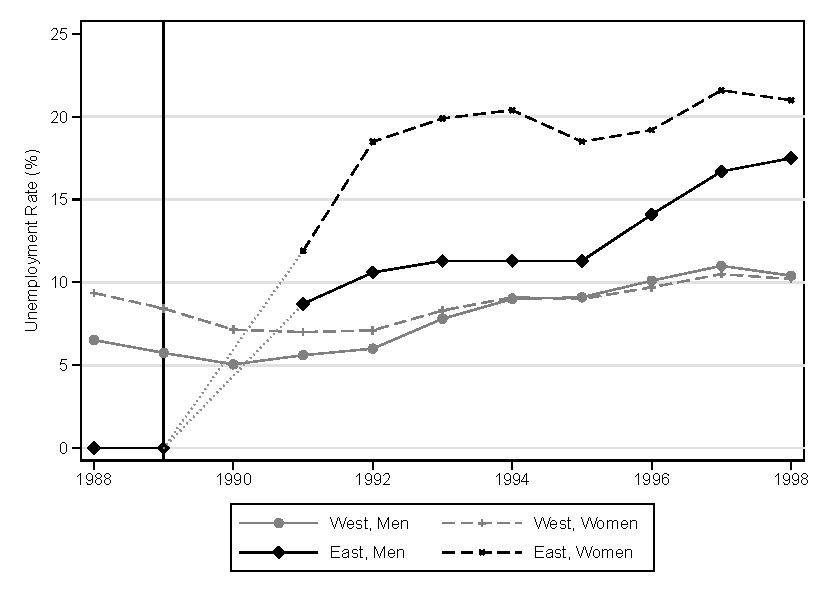
\includegraphics[scale=0.8]{UE_ASO.pdf} 
    \sourcefigure{Federal Employment Agency, various years.}
\end{figure}
%\newpage
%==================================================================%

When investigating occupational mobility in these years and assessing how unusual those years were for the GDR workforce, it is important to understand occupational mobility patterns during GDR times. To the best of my knowledge, the main source of information concerning the rates and patterns of occupational mobility during GDR times comes from the East German Life History Study (EGLHS) of the Max Planck Institute for Human Development and Education in Berlin. \cite{HuininkSolga1994} analyze the pattern of occupational mobility of four cohorts of GDR citizens born in 1929-31, 1939-41, 1951-53, and 1959-61 by comparing their occupational structure at age 30. During GDR times, job mobility could have resulted from modernization and industrialization. However, owing to central planning and state-governed labor force allocation, socialist societies are often characterized as being immobile (a notion that is consistent with the patterns shown in Figure \ref{Fig1a} discussed above). 

\cite{HuininkSolga1994} show, however, that the aggregate figures hide important heterogeneity across birth cohorts. Birth cohorts differed in age when they were subject to the different political and economic developments of the former GDR. Huinink and Solga differentiate three major periods:\footnote{I follow the categorization in \cite{HuininkSolga1994}. More detailed descriptions of the GDR system and its different phases can be found, for example, in \cite{Ritschl1995}.} (1) the period of the revolutionary implementations of the state-socialist system (from the end of World War II to the early 1960s), (2) the period of extensive economic growth connected with attempts at decentralization (the 1960s), and (3) the period of re-centralization of the economy (after Honecker came to power in 1971).

In the first phase, the roots of Nazi Germany were dismantled by introducing new rules and political measures to eliminate the old political, economic, and also bourgeois intellectual elites. These political measures included expropriation, abolishing civil servant status, and denazification. The teachers, lawyers, and civil servants, among other status groups of the previous regime, were ``downgraded'' and replaced by people loyal to the new system. During this period, labor scarcity was a widespread challenge for the GDR. This was not only due to the purging of pre-war personnel and the establishment of a new socialist administration but also because approximately 1.9 million people left the GDR for West Germany. This exodus only ended in 1961 with the construction of the Berlin Wall.\footnote{See, e.g., \cite{BlackLiepmannRemigereauSpitzOener2022}, and studies cited there.} Overall, this period was characterized by general scarcity of labor and resulted in an improvement in the occupational opportunities of men who started from lower levels of qualification, which was consistent with the political goal of creating the GDR as a ``state of workers and farmers''.

The second phase started in the 1960s, and it was characterized by the system's attempt to make the economy more efficient by following a decentralization strategy (the so-called ``Neues \"Okonomisches System, N\"OS, ``New Economic System''). During this period, access to education improved considerably, and the political system ensured a smooth transition from schools to the labor market by requiring and offering everyone a place in the vocational training system. Despite its initial positive effects on economic growth, the N\"OS fell overall short in improving the GDR economy, a fact that led to the third phase.

The third phase is associated with Erich Honecker's coming to power in 1971, which again changed the GDR's economic goals. One of the main measures was the re-centralization of the GDR economy, characterized, among other things, by the establishment of the Kombinate—large state-owned conglomerates covering the majority of an industry's plants. It was also a period in which the opportunities for higher education were reduced, and more generally, the state took an important role in labor allocation.

\cite{HuininkSolga1994} show that the opportunities to improve their occupational position that the earliest birth cohort benefitted from presented themselves to a much smaller degree to those born later, with upward occupational mobility being generally tight to system loyalty displayed by party membership or the taking on of official functions in a pro-party organization. By focusing on the occupational achievements when cohort members were 30 years old, \cite{HuininkSolga1994} show that intra-cohort mobility between the different birth cohorts was very different in the GDR. They do not investigate occupational mobility in the context of the ``Wende,'' which is the main focus of this study.

The cohort-based approach followed by \cite{HuininkSolga1994} is interesting because it allows for comparing GDR and FRG workers in 1989 who are from the same birth cohorts. Methodologically, this comparison allows netting out macro-economic factors that affected the occupational mobility of workers of different ages to a similar degree between 1989 and 1992, independent of whether they lived in the GDR or the FRG in 1989. 

However, it is also interesting to consider the differences and similarities of the different birth cohorts depending on where they were born. Based on \cite{Ritschl1995} and \cite{EichengreenRitschl2009}, I give a brief overview of the differential economic and social environments to which the different cohorts were subjected. 

One striking fact is that the 1929-31 cohort shared the same political and economic environment at birth and early childhood. This cohort was born before World War II (WWII) when Germany was still united. It was born during the early years of the Great Depression (1929-1932), a period of severe economic downturn that deeply affected all regions in Germany.\footnote{See, e.g., \cite{Schnabel2004}.} This cohort was subject to vast economic instability, high unemployment rates, and widespread poverty during their early childhood. The cohort lived under the same political and economic system until WWII ended in 1945 when they were about 15 years old. Then, the macro environment of the GDR and FGR members of this cohort diverged drastically, however, with the division into East and West Germany and the beginning of the Cold War. Those in the East faced a socialist regime under Soviet influence, while those in the West saw the establishment of a democratic state and economic recovery. The West German members of this cohort experienced the period of the  Wirtschaftswunder (Economic Miracle) in West Germany of the 1950s and 1960s when they were of prime working age. Overall, the political and economic environment differed vastly for the GDR and FRG members of the 1929-31 cohort after 1945.

The 1939-41 cohort was born during the early years of World War II. As infants and toddlers, they were exposed to the immediate impacts of the war, including air raids, displacement, and general instability. They were in their early childhood when they experienced the destructive consequences of the war and the division of Germany. Their formative years coincided with the immediate post-war period, characterized by massive reconstruction efforts and economic hardship. West Germany's Wirtschaftswunder began in the late 1940s and accelerated in the 1950s, providing improving living conditions and economic opportunities as they reached adolescence and young adulthood. This cohort benefited from increased access to education, which was a crucial factor in the country's rapid economic recovery. Socialization in this period was also marked by strongly emphasizing democratic principles and rejecting totalitarian ideologies.

Members of the 1951-53 cohort were among the first to be born in the two divided states founded in 1949, the GDR and FRG. Both states underwent a period of significant reconstruction and recovery. In the West, this era is characterized by the booming economy and an expansion of the welfare state, leading to rapid economic growth and rapidly increasing living standards. In East Germany, the members of this cohort grew up in phases (1) and (2) described above. Independent of whether they grew up in the East or the West, because of their early birth, the members experienced all phases of political and economic development from the period of division to reunification. They reached adulthood when the Cold War was the characterizing policy between the East and the West. 

The 1959-61 cohort was born during a period of heightened Cold War tensions. The Berlin Wall, erected in 1961, symbolized the division they were born into, significantly impacting their early years. In West Germany, they experienced a society focused on economic growth and integration with Western Europe and Western countries more generally, while in East Germany, they lived under a socialist regime with a state-controlled economy, limited political freedoms, and strong political and economic connections to the Soviet Union. 


%====================================================================%
\section{Data and Variables}\label{data}
\subsection{Data on GDR Workers}\label{GDRdata}
The novel, individual-level administrative data set on GDR workers used in this study is the result of linking data from the so-called ``Data Fund of Societal Work Power'' of the GDR (``Datenspeicher Gesellschaftliches Arbeitsvermögen (GAV)'' in German), obtained from the Federal Archive in Germany, with the so-called ``Integrated Employment Biographies'' (IEB data). The former provides information on the demographics and labor market characteristics of around 7 million persons in the GDR in 1989, representing the near universe of workers in the GDR. The latter contains the complete employment and earnings histories of all workers covered by the social security system in Germany from 1975 onward. The two data sets were merged on names, exact dates of birth, and gender. The combined data allows for addressing questions regarding mobility across jobs, occupations, and migration decisions after German reunification while also providing labor market information on GDR workers during GDR times.\footnote{A detailed description of the data sources and linkage can be found in \parencite{LiepmannMuller2018}.} 


%====================================================================%
\subsection{Data on FRG Workers}
For information on the cohorts born in the FRG, I rely on the Sample of Integrated Labor Market Biographies (SIAB) of the Institute for Employment Research (IAB). It is a 2\% random sample drawn from the IEB, the database to which the GDR workers were merged, as described above. It provides high-quality information on the labor market trajectory of workers, including information on the occupation, employer, and gross daily wages. In the context of this study, I selected all employed men and women of the relevant birth cohorts in the FRG 1989, including full- and part-time workers (the sample includes about 12\% part-time workers). In contrast to the sample described in \ref{GDRdata}, which includes the near universe of GDR workers, I rely on a 2\% random sample of FRG workers for efficiency reasons. This explains the differences in sample size shown below. 

%====================================================================%
\subsection{Main Variables}

To be able to compare the occupational structure in the two very different economic systems of the GDR and FRG, I use a variant of the so-called Blossfeld occupational categories that categorize occupations into 6 categories, depending on socio-economic status. The six broad categories allow for comparing the occupational structure of two states with very different economic systems. This also allows comparing the results with previous findings in \cite{MayerSolga1994} and \cite{HuininkSolga1994}, among others. Table \ref{tab1} shows the categories. The first category, ``Professional and higher technical, administrative, managerial occupations,'' includes engineers, technicians, managers, and senior government officials. The second category, ``Semiprofessional occupations,'' includes journalists, translators, librarians, and teachers. The third category, ``Skilled workers,'' includes craftsmen, mechanics, bakers, butchers, and brewers. The fourth category, ``Unskilled workers,'' includes assemblers, building laborers, packagers, and dispatchers. The fifth category, ``missing employment information,'' is somewhat of a residual, including, for example, non-agricultural family assistants, trainees, and interns without specified occupations. This category is probably closest to category (4), ``unskilled workers.'' The sixth category, ``non-employed,'' includes non-employed workers.

Regarding occupational mobility between 1989 and 1992, "upward mobility" is defined as moving into a lower numerical category, such as from 3 to 1; ``downward mobility'' is defined as moving into a higher numerical category, such as from 1 to 3. ``Movement to non-employment'' is defined as moving from any non-level 6 category in 1989 to category 6 in 1992. ``Lateral mobility'' is defined as movements between occupations that are in the same category, and ``non-movement'' is defined as staying in the same 2-digit occupation. Note that this classification completely ignores regional mobility. For example, a person who stayed in the same 2-digit occupation is part of the  ``non-movement'' category even though they might have moved from Rostock to Mannheim.

%====================================================================%

\begin{table}[h!]
\caption{Employment Categories}\label{tab1}
\centering
\begin{tabular}{cl}
\toprule
Number & Category \\
\midrule
1 & Professionals, and higher technical, administrative, \\
  & and managerial occupations \\ 
2 & Semiprofessional occupations \\ 
3 & Skilled workers \\ 
4 & Unskilled workers \\
5 & Missing employment information \\ 
6 & Non-employed \\ \bottomrule
\end{tabular}
\end{table}

%==================================================================%

\clearpage
I consider three different levels of education: the low-educated have no vocational training degree, the medium-educated have a degree through the dual system of apprenticeship or a vocational school, and the high-educated have a degree from a university or a technical college. Because of the joint historical roots of the education system in the two parts of Germany, this variable is easy to construct for GDR and FRG workers.



%====================================================================%
\section{The Status Quo in 1989}\label{StatusQuo}

Using information about education and occupational structure, I will first compare the GDR and FRG labor market in 1989, i.e., when the Berlin Wall fell. Table \ref{tab2} shows summary statistics for the 4 birth cohorts (1929-31, 1939-41, 1951-1953, 1959-61) for GDR workers (Panel A) and FRG workers (Panel B) in 1989, separately by gender. It is important to note that, by fixing the year to 1989 and looking at different cohorts, we are comparing demographic groups of different ages in 1989. The oldest cohort was, on average, 60 years old in 1989, the 1939-41 cohort was 49, the 1951-53 cohort was 37, and the 1959-61 cohort was 29 years old in 1989. Differences across cohorts might, therefore, reflect age effects. This is not the case when discussing results for the same birth cohort across demographic groups (men and women in the GDR or FRG), as members of the same birth cohort across groups were of the same age in 1989.\footnote{\cite{HuininkSolga1994} fix the age to 30 when comparing the different cohorts.}

%=======================================================%
%\vspace{1cm}   
\begin{table}[!ht]
\caption{Summary Statistics in 1989}\label{tab2}
\centering
\resizebox{\textwidth}{!}{
\begin{tabular}{lrrrrrrrrrr}
\toprule
\multicolumn{2}{l}{\textbf{Panel A: GDR Workers}} & \multicolumn{9}{c}{\textbf{}}\\ [0.1cm]
\cline{1-11}
 &  &  &  &  &  &  &  &  &  &  \\
\multicolumn{1}{l}{\textbf{}} & \multicolumn{5}{c}{\textbf{Men}} & \multicolumn{5}{c}{\textbf{Women}} \\ [0.3cm]
%\cline{1-11} 
\multicolumn{1}{l}{\textbf{Birth cohort:}} & {\textbf{1929-31}} & \multicolumn{1}{c}{\textbf{1939-41}} & {\textbf{1951-53}} & {\textbf{1959-61}} & \multicolumn{1}{c}{\textbf{all}} & {\textbf{1929-31}} & {\textbf{1939-41}} & {\textbf{1951-53}} & {\textbf{1959-61}} & \multicolumn{1}{c}{\textbf{all}} \\ \midrule
\multicolumn{1}{l}{Share (in\%)} & \multicolumn{10}{c}{} \\ 
... low educated  & {74.5} & {11.4} & {8.4} & {8.1} & {15.9} & {45.6} & {22.8} & {11.0} & {9.6} & 14.9 \\ 
\multicolumn{1}{l}{... medium educated} & {19.3} & {74.6} & {79.5} & {84.4} & {73.4} & {51.1} & {72.4} & {79.2} & {82.4} & 77.7 \\ 
\multicolumn{1}{l}{... higher educated} & {6.2} & {14.0} & {12.1} & {7.4} & {10.6} & {3.3} & {4.9} & {9.8} & {8.0} & 7.4 \\
 ... in occupation group (1)  & {7.8} & {8.5} & {6.5} & {5.1} & {6.8} & {4.7} & {6.8} & {11.7} & {11.8} & 10.0 \\ 
... in occupation group (2)  & {0.9} & {0.6} & {0.4} & {0.3} & {0.5} & {5.4} & {6.4} & {8.2} & {9.2} & 7.9 \\ 
... in occupation group (3)  & {48.6} & {51.0} & {54.3} & {54.1} & {52.7} & {22.2} & {25.7} & {31.3} & {28.7} & 28.5 \\ 
... in occupation group (4) & {29.4} & {27.1} & {26.4} & {25.4} & {26.6} & {35.0} & {40.0} & {35.4} & {38.9} & 38.1 \\
... in occupation group (5)  & {13.3} & {12.9} & {12.3} & {15.2} & {13.5} & {32.6} & {21.1} & {13.3} & {11.4} & 15.5 \\ [0.2cm]
Average Age \\ (Std. Dev.) & {\begin{tabular}[t]{@{}r@{}}58.6\\ (0.75)\end{tabular}} & {\begin{tabular}[t]{@{}r@{}}49.0\\ (0.81)\end{tabular}} & {\begin{tabular}[t]{@{}r@{}}37.0\\ (0.82)\end{tabular}} & {\begin{tabular}[t]{@{}r@{}}29.0\\ (0.82)\end{tabular}} & {\begin{tabular}[t]{@{}r@{}}40.4\\ (9.99)\end{tabular}} & {\begin{tabular}[t]{@{}r@{}}58.8\\ (0.79)\end{tabular}} & {\begin{tabular}[t]{@{}r@{}}49.0\\ (0.81)\end{tabular}} & {\begin{tabular}[t]{@{}r@{}}37.0\\ (0.82)\end{tabular}} & {\begin{tabular}[t]{@{}r@{}}29.0\\ (0.82)\end{tabular}} & \begin{tabular}[t]{@{}r@{}}38.7\\ (8.53)\end{tabular} \\[0.5cm]
\multicolumn{1}{l}{Number of Observations} & {81,137} & {241,047} & {233,329} & {242,806} & {798,319} & {5,777} & {215,961} & {199,821} & {208,266} & 629,825 \\ \bottomrule
 &  &  &  &  &  &  &  &  &  &  \\
 &  &  &  &  &  &  &  &  &  &  \\
\multicolumn{2}{l}{\textbf{Panel B: FRG Workers}} & \multicolumn{9}{c}{\textbf{}}\\ [0.1cm]
\cline{1-11}
 &  &  &  &  &  &  &  &  &  &  \\
\multicolumn{1}{l}{\textbf{}} & \multicolumn{5}{c}{\textbf{Men}} & \multicolumn{5}{c}{\textbf{Women}} \\ [0.3cm]
%\cline{1-11} 
\multicolumn{1}{l}{\textbf{Birth cohort:}} & {\textbf{1929-31}} & {\textbf{1939-41}} & {\textbf{1951-53}} & {\textbf{1959-61}} & \multicolumn{1}{c}{\textbf{all}} & {\textbf{1929-31}} & {\textbf{1939-41}} & {\textbf{1951-53}} & {\textbf{1959-61}} & \multicolumn{1}{c}{\textbf{all}} \\ \midrule
\multicolumn{1}{l}{Share (in\%)} & \multicolumn{10}{c}{} \\
... lower educated  & {62.1} & {25.0} & {18.6} & {21.3} & {27.1} & {88.6} & {39.8} & {31.0} & {40.0} & 42.9 \\ 
\multicolumn{1}{l}{... medium educated} & {32.9} & {67.2} & {68.4} & {68.3} & {63.4} & {10.7} & {58.0} & {63.5} & {53.1} & 52.7 \\ 
\multicolumn{1}{l}{... high educated} & {5.0} & {7.7} & {12.9} & {10.3} & {9.5} & {0.7} & {2.3} & {5.4} & {6.9} & 4.4 \\ 
... in occupation group (1) & {19.5} & {19.8} & {19.2} & {15.5} & {18.3} & {3.3} & {4.3} & {6.5} & {9.6} & 6.5 \\ 
... in occupation group (2) & {1.4} & {1.3} & {2.8} & {2.3} & {2.0} & {6.0} & {6.0} & {9.6} & {13.0} & 9.2 \\ 
... in occupation group (3) & {35.4} & {37.0} & {42.5} & {43.6} & {40.2} & {32.4} & {37.4} & {40.9} & {43.3} & 39.7 \\ 
... in occupation group (4) & {43.8} & {41.9} & {35.5} & {38.6} & {39.5} & {58.3} & {52.2} & {42.9} & {34.1} & 44.7 \\ [0.2cm]
Average Age \\ (Std. Dev.) & {\begin{tabular}[t]{@{}r@{}}58.8\\ (0.80)\end{tabular}} & {\begin{tabular}[t]{@{}r@{}}49.01\\ (0.81)\end{tabular}} & {\begin{tabular}[t]{@{}r@{}}37.0\\ (0.81)\end{tabular}} & {\begin{tabular}[t]{@{}r@{}}29.0\\ (0.82)\end{tabular}} & {\begin{tabular}[t]{@{}r@{}}41.0\\ (10.51)\end{tabular}} & {\begin{tabular}[t]{@{}r@{}}58.8\\ (0.78)\end{tabular}} & {\begin{tabular}[t]{@{}r@{}}49.0\\ (0.81)\end{tabular}} & {\begin{tabular}[t]{@{}r@{}}37.0\\ (0.82)\end{tabular}} & {\begin{tabular}[t]{@{}r@{}}29.0\\ (0.82)\end{tabular}} & \begin{tabular}[t]{@{}r@{}}40.5\\ (10.28)\end{tabular} \\ [0.5cm]
\multicolumn{1}{l}{Number of Observations} & {8,769} & {20,561} & {17,196} & {21,025} & {67,551} & {4,462} & {12,850} & {10,660} & {13261} & 41,233 \\ \bottomrule
\end{tabular}}

\vspace{0.3cm}
\parbox[h]{\linewidth}{\footnotesize{Note: The table shows summary statistics for workers of the German Democratic Republic (GDR) and the Federal Republic of Germany (FRG) in 1989. See Section \ref{data} for details on the data and definition of variables.}}
\end{table}
%\end{landscape}
%\vspace{1cm}

%======================================%

As discussed above, the oldest cohort (born 1929-31) is interesting, as they were born and grew up under the same political and economic system until the end of WWII, when they were about 15 years old. Note surprisingly, in terms of formal education, it is the least educated cohort. 74.5\% of the GDR men of this cohort had low levels of education in 1989, while this figure was considerably lower at 62\% for FRG men of this cohort. In contrast, the share of medium educated was considerably higher for FGR men of this cohort compared to their GDR counterparts. The share of highly educated was quite similar, with 6.2\% for GDR men and 5.0\% for FRG men. 

Regarding women, it is important to note that labor force participation at about 43\% was relatively low in the FRG in 1989, whereas the estimates for the GDR are around 80-90\%. As a result, working women in the FRG were much more selective than in the GDR. Against this background, the differences in formal education are striking between women in the GDR and FRG. While only about 46\% of GDR women in the oldest cohort had low levels of education, this figure was 89\% for FRG women. In addition, 51\% of GDR women had a medium level of education, compared to only 11\% of FRG women. More than 3\% of GDR women in this cohort even had a degree from a university or a technical college.  

For the subsequent cohorts and both genders, the educational structure typical for the German labor market is visible in both groups, with men and women of medium education making up the largest shares. Overall, the across-cohort patterns show that educational upgrading was large for both genders and in both parts of Germany up to 1989. When comparing the two youngest cohorts of GDR workers, the "Honecker" years are also visible, as the educational attainment shifted from high towards medium-educated workers.

The table also shows the distribution of employment across the 5 different occupation groups used in the previous literature and described in Table \ref{tab1}. With about 9\%, the share of ``Professional/Higher technical, administrative, managerial'' occupations (group 1) and ``Semiprofessional'' positions (group 2) among the 1929-31 cohort of GDR men was much lower than the about 21\% among FRG men. Most (about 49\%) of GDR men in this cohort worked as skilled workers (group 3), while this group comprised about 35\% of FRG male workers. The share of unskilled workers in the GDR was about 30\%, and about 13.5\% of workers were not assignable to one of the categories (a detailed look at the occupations suggests, however, that they are closest to the unskilled group). In the FRG, the share of unskilled male workers was about 44\%, comparable to that of GDR workers in occupation groups (4) and (5) combined. 

Regarding women of this oldest cohort in the FRG and GDR, the share in the highest occupational categories is not dramatically different, with about 10\% in the GDR and about 9\% in the FRG. The share of women working as skilled workers is about 10 percentage points higher in the FRG than in the GDR. 58\% of FRG women worked as unskilled workers (group 4), whereas this is only the case for 35\% of GDR female workers. However, the latter increases by 32 percentage points if one counts the relatively high share of GDR female workers who cannot be unambiguously assigned to either of the categories to the unskilled category. 

Looking across cohorts, the younger the women are, the higher the employment share of the two highest occupational categories (groups 1 and 2). Among the GDR female workers born between 1959 and 1961, 21\% worked in these two occupational categories, whereas this was the case for about 23\% of FRG female workers. About 29\% of female GDR workers were employed as skilled workers, compared to more the 43\% of FRG female workers of this cohort. With about 39\%, the share of female GDR workers who worked as unskilled workers was about 5 percentage points higher than for female FRG workers. In addition, about 11\% of GDR women worked in occupation categories (5) that are also closest to the unskilled category. 

Overall, it is striking that GDR women's better educational attainment did not result in higher shares of employment in higher occupational categories (groups 1 to 3), a pattern that also applies to men (but is less pronounced).


%====================================================================%
\section{Occupational Mobility of GDR Workers Between 1989 and 1992}\label{1989to1992}

How did the first years of transition affect the occupational mobility of the different GDR cohorts? To disentangle the effects of the ``Wende'' from the economic effects that Germany was subject to at the beginning of the 1990s and that affected different cohorts in the same way in East and West Germany, I compare the occupational mobility of GDR workers with that of West Germans from the same birth cohort.

Figure \ref{fig3} displays the differences in employment mobility between 1989 and 1992 of GDR and FRG male workers. Differences in upward, lateral downward, movement-to-non-employment, and non-mobility shifts are displayed with one bar representing each type of mobility for each of the four cohorts considered (1929-31, 1939-41, 1951-53, 1959-61) and across all cohorts. As the difference is taken between GDR and FRG male workers, bars above the x-axis indicate a greater share for GDR than FRG, and bars below the x-axis indicate a smaller share for GDR than FRG male workers. The underlying data, separately for GDR and FRG workers by gender, are shown in Table \ref{tab3}.

\pagebreak

Between 1989 and 1992, male GDR workers of the 1929-1931 birth cohort were 5.6 percentage points more likely to move upward than FRG workers of the same cohort (first bar) and 3.7 percentage points more likely to move to an occupation within the same status category (fourth bar from left); however, they were also 3.3 percentage points more likely to move downward, and about 26 percentage points more likely to move into non-employment. The largest difference exists for non-mobility, with FRG male workers of this cohort being 40 percentage points more likely to stay in the same occupation than GDR workers of this cohort.

Regarding men born between 1939 and 1941 (aged 48-50 in 1989), the GDR men were about 25 percentage points more likely to move upward (first bar in the second cluster of bars) and about 20 percentage points more likely to move to occupations within the same status group than FRG men between 1989 and 1992. However, they are also about 17 percentage points more likely to move downward. With a difference of only 1.4 percentage points, GDR and FRG men of this cohort were about equally likely to move to non-employment. The biggest difference, again, is for non-mobility, where FRG workers are about 63 percentage points more likely to stay in the same occupations than GDR workers.

The overall pattern is very similar for men born from 1951 to 1953 and those born from 1959 to 1961, with all mobility categories being larger for GDR workers than FRG workers. Again, the difference in movement to non-employment is small relative to the differences in other categories; again, the FRG workers are much more likely to remain in the same occupation as the GDR workers. In contrast to the high emphasis typically placed on unemployment regarding labor market developments of GDR workers, for all birth cohorts, except for 1929 to 1931, the largest difference between GDR and FRG male workers is occupational mobility versus occupational stability between 1989 and 1992.

Figure \ref{fig4} shows the differences in employment mobility between 1989 and 1992 of GDR and FRG female workers. The pattern for the oldest cohort, born 1929 to 1931, looks quite different for women than for men. Most strikingly, the share of women moving into non-employment is larger among FRG than GDR women by about 32 percentage points. This is not only different from what is observed for men but also compared to the pattern of all other female cohorts. In contrast, the difference in non-mobility is much smaller for this birth cohort. Upward mobility is about 23 percentage points higher, and lateral mobility is about 12 percentage points for GDR than FRG women of this cohort, whereas downward mobility is about 9 percentage points higher.

Looking across female cohorts, upward mobility is always larger than downward mobility, suggesting that the opportunities for occupational upgrading were larger for GDR women between 1989 and 1992 than for FRG women and compared to the risk of downgrading. However, GDR women also had a higher probability of moving into non-employment. Similar to what is observed for men, for all birth cohorts, except for 1929 to 1931, the largest difference between GDR and FRG male workers is occupational mobility versus occupational stability between 1989 and 1992. 

%====================================================================%
\begin{landscape}
    
\begin{figure}[!ht]
    \caption{\textbf Distribution of East-West Differences in Occupational Shifts between 1989 and 1992 for Selected Birth Cohorts, Men}\label{fig3}
%    \vspace{-0.5cm}
    \begin{center}
    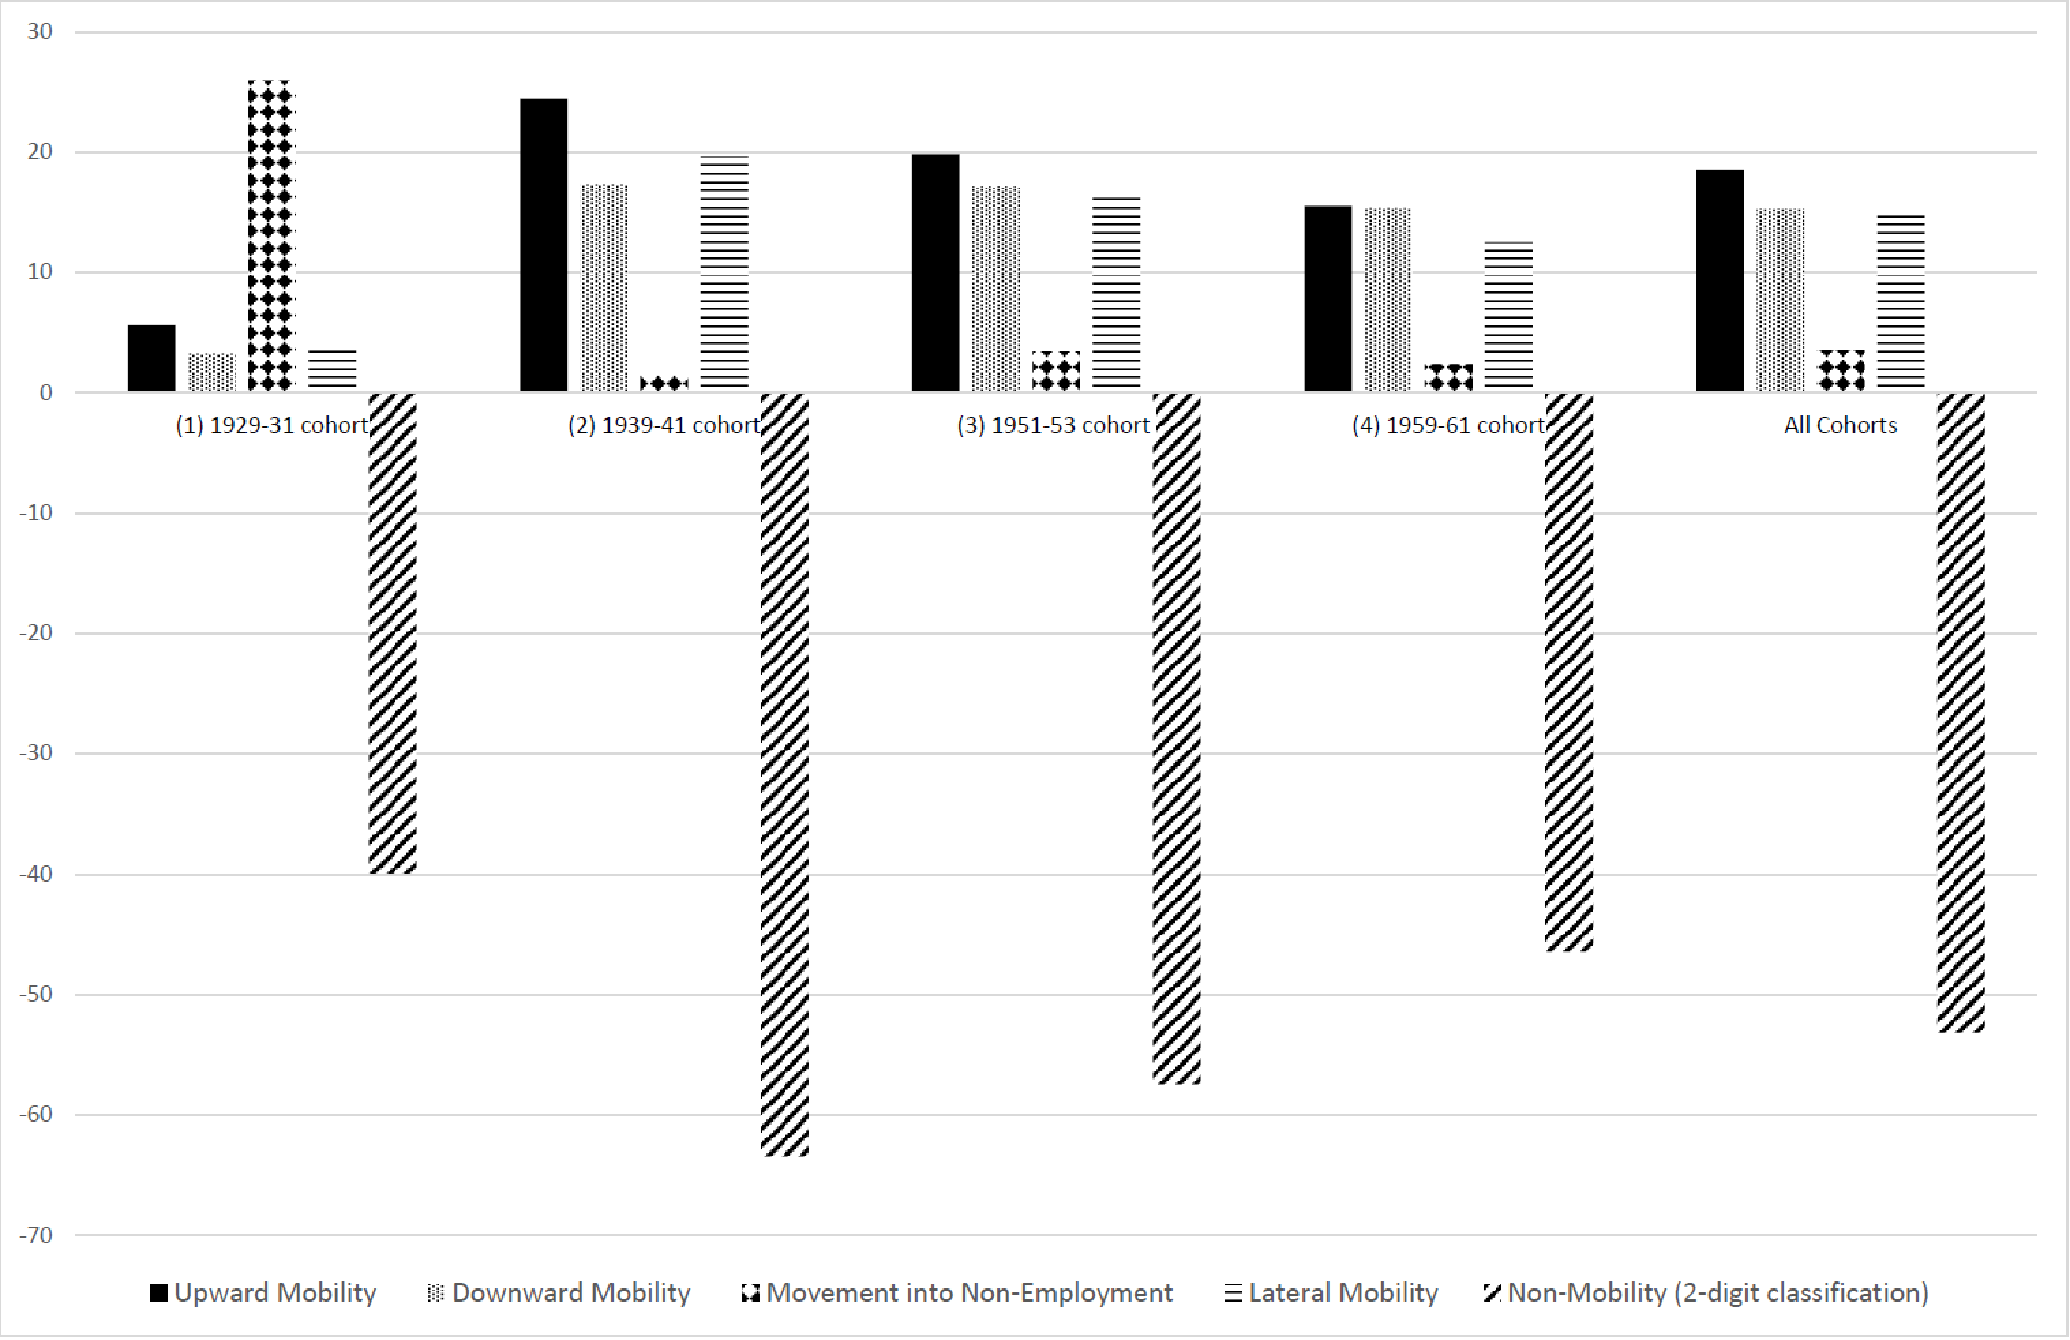
\includegraphics[width=.8\linewidth]{East_vs_West_Men.pdf}
    \vspace{-3.8cm}
    {\footnotesize
    \hspace*{0.1cm}\parbox[h]{\linewidth}{Notes: The figure shows the differences in the shares of occupational mobility of GDR and FRG male workers between 1989 and 1992, separately by birth cohort and overall. ``Upward mobility" is defined as moving into a lower numerical category, such as from 3 to 1 (see Table \ref{tab1}); ``downward mobility'' is defined as moving into a higher numerical category, such as from 1 to 3. ``Movement to non-employment'' is defined as moving from any non-level 6 category in 1989 to category 6 in 1992. ``Lateral mobility'' is defined as movements between occupations that are in the same category, and ``non-movement'' is defined as staying in the same 2-digit occupation.}}
    \end{center}
\end{figure}
\end{landscape}


%====================================================================%
\begin{landscape}
    
\begin{figure}[!ht]
    \caption{\textbf Distribution of East-West Differences in Occupational Shifts between 1989 and 1992 for Selected Birth Cohorts, Women}\label{fig4}
%    \vspace{-0.5cm}
    \begin{center}
    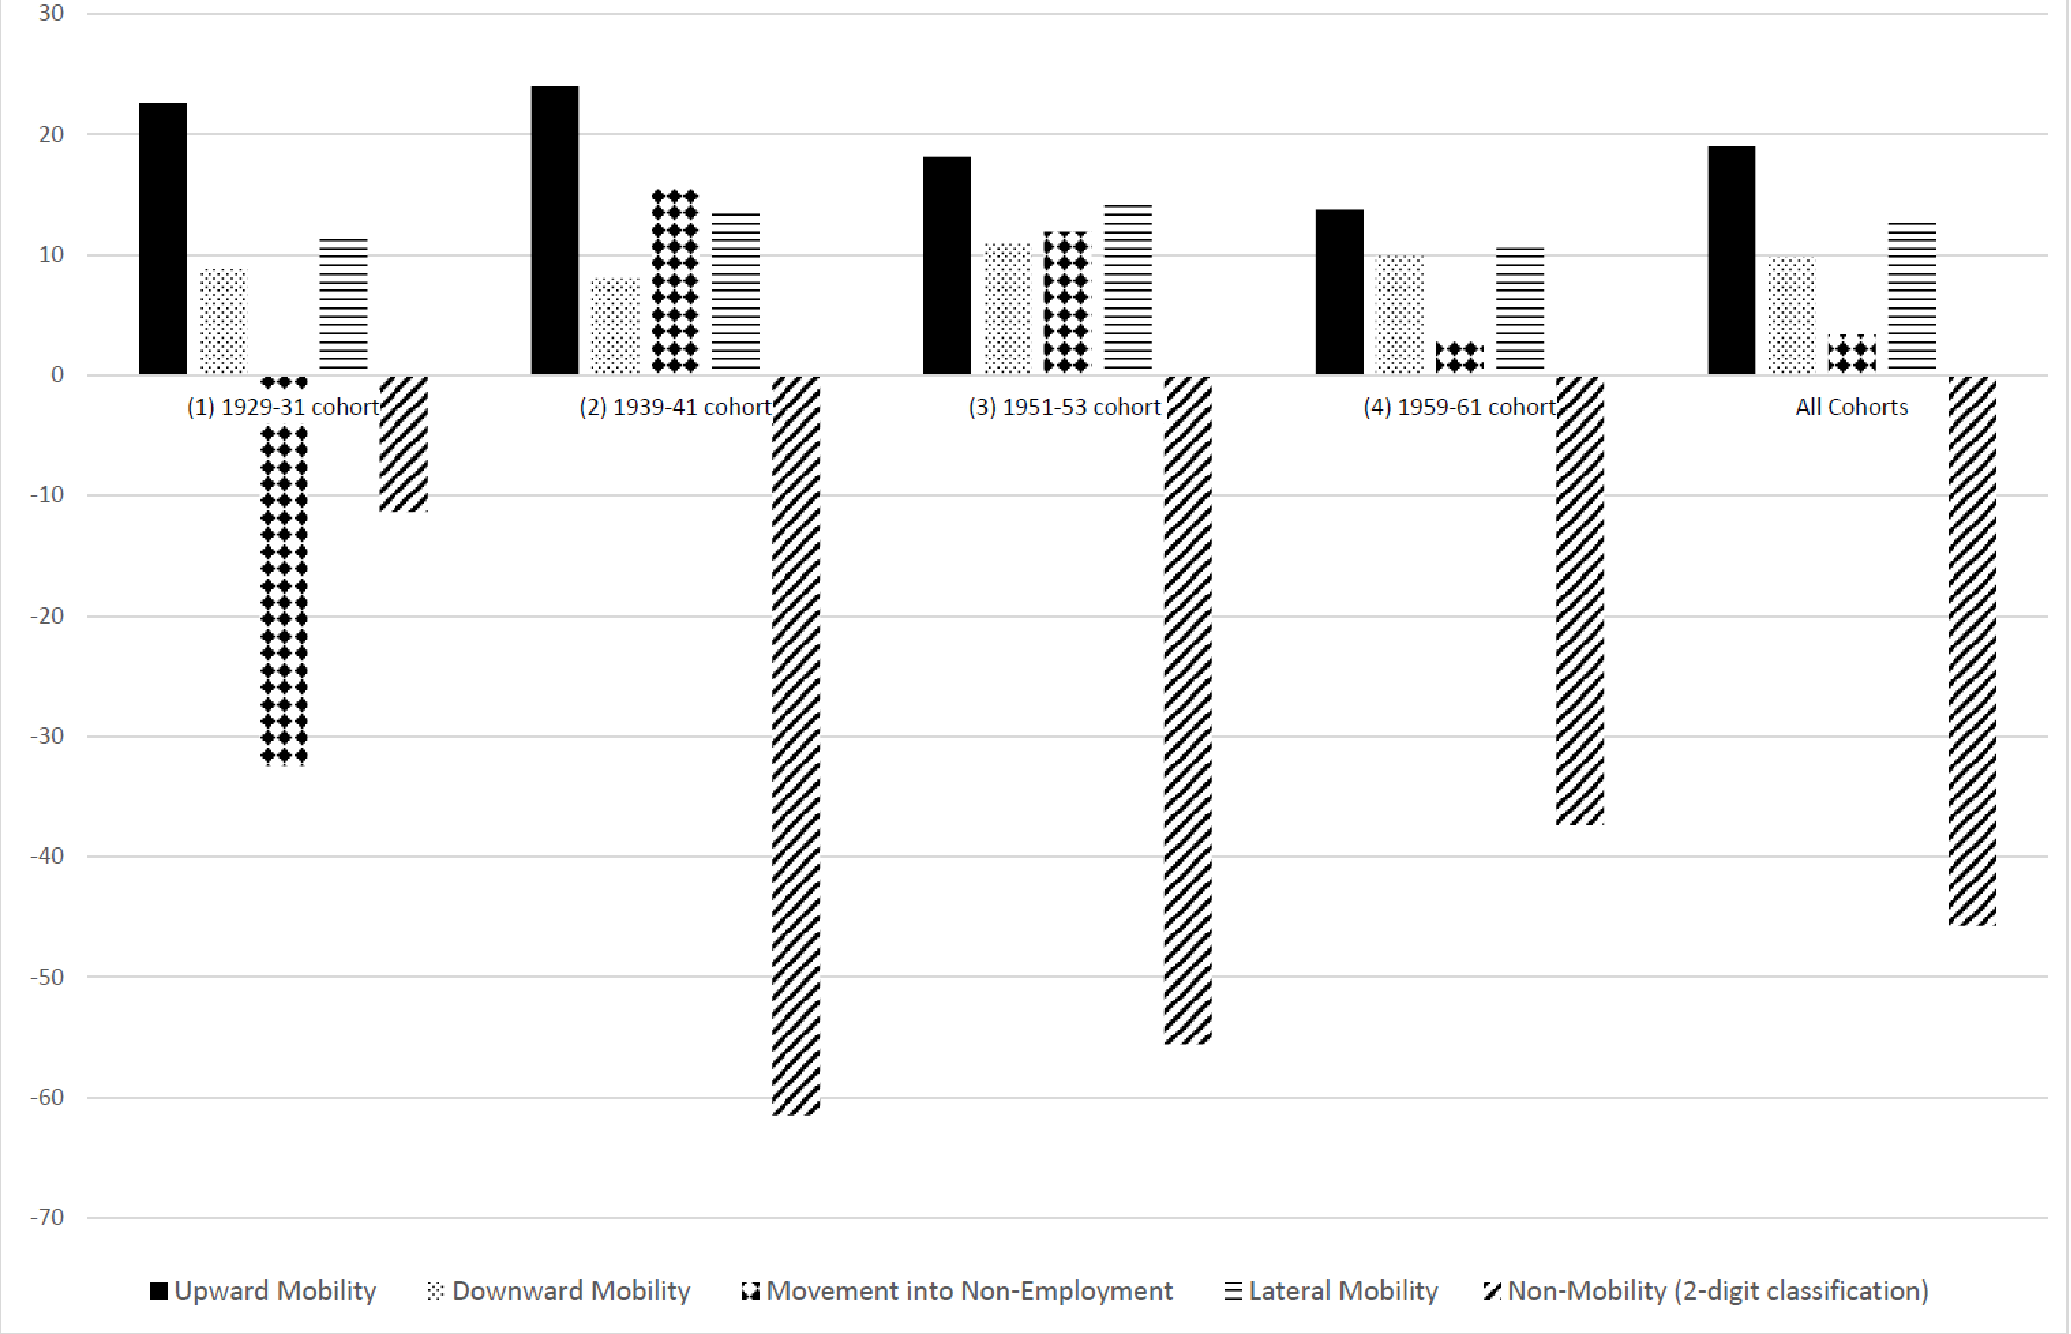
\includegraphics[width=.8\linewidth]{East_vs_West_Women.pdf}
    \vspace{-3.8cm}
    {\footnotesize
    \hspace*{0.1cm}\parbox[h]{\linewidth}{Notes: The figure shows the differences in the shares of occupational mobility of GDR and FRG female workers between 1989 and 1992, separately by birth cohort and overall. ``Upward mobility" is defined as moving into a lower numerical category, such as from 3 to 1 (see Table \ref{tab1}); ``downward mobility'' is defined as moving into a higher numerical category, such as from 1 to 3. ``Movement to non-employment'' is defined as moving from any non-level 6 category in 1989 to category 6 in 1992. ``Lateral mobility'' is defined as movements between occupations that are in the same category, and ``non-movement'' is defined as staying in the same 2-digit occupation.}}
    \end{center}
\end{figure}
\end{landscape}

%---------------------------------------------------------%
\begin{landscape}
\begin{table}[]
\centering
\caption{Occupational Mobility between 1989 and 1992}\label{tab3}
% \vspace{-0.2cm}
\resizebox{12cm}{!}{%
\begin{tabular}{lll*5{r}}
\hline
\multicolumn{1}{r}{} & \multicolumn{1}{r}{\textbf{Sex}} & \multicolumn{1}{r}{\textbf{Cohort}} & \multicolumn{1}{r}{\textbf{Upward Mobility}} & \multicolumn{1}{r}{\textbf{Downward Mobility}} & \multicolumn{1}{r}{\textbf{\begin{tabular}[t]{@{}r@{}}Movement into \\ Non-Employment\end{tabular}}} & \multicolumn{1}{r}{\textbf{\begin{tabular}[t]{@{}r@{}}Lateral Mobility \end{tabular}}} & \textbf{\begin{tabular}[t]{@{}r@{}}Non-Mobility \\ (2-digit classification)\end{tabular}} \\ \hline
\multicolumn{1}{r}{\multirow{10}{*}{\textbf{GDR Workers}}} & \multicolumn{1}{r}{\multirow{5}{*}{Men}} & \multicolumn{1}{l}{(1) 1929-31 cohort} & \multicolumn{1}{r}{7.7} & \multicolumn{1}{r}{3.7} & \multicolumn{1}{r}{80.2} & \multicolumn{1}{r}{4.7} & 3.6 \\ \cline{3-8} 
\multicolumn{1}{r}{} & \multicolumn{1}{r}{} & \multicolumn{1}{r}{(2) 1939-41 cohort} & \multicolumn{1}{r}{26.8} & \multicolumn{1}{r}{19.2} & \multicolumn{1}{r}{14.1} & \multicolumn{1}{r}{23.3} & 16.4 \\ \cline{3-8} 
\multicolumn{1}{r}{} & \multicolumn{1}{r}{} & \multicolumn{1}{r}{(3) 1951-53 cohort} & \multicolumn{1}{r}{24.1} & \multicolumn{1}{r}{20.1} & \multicolumn{1}{r}{15.0} & \multicolumn{1}{r}{22.0} & 18.5 \\ \cline{3-8} 
\multicolumn{1}{r}{} & \multicolumn{1}{r}{} & \multicolumn{1}{r}{(4) 1959-61 cohort} & \multicolumn{1}{r}{21.9} & \multicolumn{1}{r}{19.5} & \multicolumn{1}{r}{16.2} & \multicolumn{1}{r}{21.0} & 21.2 \\ \cline{3-8} 
\multicolumn{1}{r}{} & \multicolumn{1}{r}{} & \multicolumn{1}{r}{All Cohorts} & \multicolumn{1}{r}{22.6} & \multicolumn{1}{r}{18.0} & \multicolumn{1}{r}{21.7} & \multicolumn{1}{r}{20.4} & 17.2 \\ \cline{2-8} 
\multicolumn{1}{r}{} & \multicolumn{1}{r}{\multirow{5}{*}{Women}} & \multicolumn{1}{r}{(1) 1929-31 cohort} & \multicolumn{1}{r}{23.6} & \multicolumn{1}{r}{8.8} & \multicolumn{1}{r}{49.1} & \multicolumn{1}{r}{11.6} & 6.2 \\ \cline{3-8} 
\multicolumn{1}{r}{} & \multicolumn{1}{r}{} & \multicolumn{1}{r}{(2) 1939-41 cohort} & \multicolumn{1}{r}{26.5} & \multicolumn{1}{r}{9.6} & \multicolumn{1}{r}{31.6} & \multicolumn{1}{r}{16.4} & 15.6 \\ \cline{3-8} 
\multicolumn{1}{r}{} & \multicolumn{1}{r}{} & \multicolumn{1}{r}{(3) 1951-53 cohort} & \multicolumn{1}{r}{22.4} & \multicolumn{1}{r}{13.6} & \multicolumn{1}{r}{28.0} & \multicolumn{1}{r}{18.6} & 17.3 \\ \cline{3-8} 
\multicolumn{1}{r}{} & \multicolumn{1}{r}{} & \multicolumn{1}{r}{(4) 1959-61 cohort} & \multicolumn{1}{r}{18.2} & \multicolumn{1}{r}{12.8} & \multicolumn{1}{r}{34.6} & \multicolumn{1}{r}{15.6} & 18.7 \\ \cline{3-8} 
\multicolumn{1}{r}{} & \multicolumn{1}{r}{} & \multicolumn{1}{r}{All Cohorts} & \multicolumn{1}{r}{22.4} & \multicolumn{1}{r}{11.9} & \multicolumn{1}{r}{31.6} & \multicolumn{1}{r}{16.8} & 17.1 \\ \hline
\multicolumn{1}{r}{\multirow{10}{*}{\textbf{FRG Workers}}} & \multicolumn{1}{r}{\multirow{5}{*}{Men}} & \multicolumn{1}{r}{(1) 1929-31 cohort} & \multicolumn{1}{r}{2.1} & \multicolumn{1}{r}{0.5} & \multicolumn{1}{r}{54.3} & \multicolumn{1}{r}{1.0} & 43.5 \\ \cline{3-8} 
\multicolumn{1}{r}{} & \multicolumn{1}{r}{} & \multicolumn{1}{r}{(2) 1939-41 cohort} & \multicolumn{1}{r}{2.3} & \multicolumn{1}{r}{1.9} & \multicolumn{1}{r}{12.7} & \multicolumn{1}{r}{3.5} & 79.8 \\ \cline{3-8} 
\multicolumn{1}{r}{} & \multicolumn{1}{r}{} & \multicolumn{1}{r}{(3) 1951-53 cohort} & \multicolumn{1}{r}{4.3} & \multicolumn{1}{r}{3.0} & \multicolumn{1}{r}{11.6} & \multicolumn{1}{r}{5.4} & 76.0 \\ \cline{3-8} 
\multicolumn{1}{r}{} & \multicolumn{1}{r}{} & \multicolumn{1}{r}{(4) 1959-61 cohort} & \multicolumn{1}{r}{6.4} & \multicolumn{1}{r}{4.1} & \multicolumn{1}{r}{13.8} & \multicolumn{1}{r}{8.5} & 67.6 \\ \cline{3-8} 
\multicolumn{1}{r}{} & \multicolumn{1}{r}{} & \multicolumn{1}{r}{All Cohorts} & \multicolumn{1}{r}{4.1} & \multicolumn{1}{r}{2.7} & \multicolumn{1}{r}{18.2} & \multicolumn{1}{r}{5.2} & 70.3 \\ \cline{2-8} 
\multicolumn{1}{r}{} & \multicolumn{1}{r}{\multirow{5}{*}{Women}} & \multicolumn{1}{r}{(1) 1929-31 cohort} & \multicolumn{1}{r}{1.0} & \multicolumn{1}{r}{0.0} & \multicolumn{1}{r}{81.5} & \multicolumn{1}{r}{0.0} & 17.5 \\ \cline{3-8} 
\multicolumn{1}{r}{} & \multicolumn{1}{r}{} & \multicolumn{1}{r}{(2) 1939-41 cohort} & \multicolumn{1}{r}{2.5} & \multicolumn{1}{r}{1.6} & \multicolumn{1}{r}{16.1} & \multicolumn{1}{r}{2.8} & 77.1 \\ \cline{3-8} 
\multicolumn{1}{r}{} & \multicolumn{1}{r}{} & \multicolumn{1}{r}{(3) 1951-53 cohort} & \multicolumn{1}{r}{4.2} & \multicolumn{1}{r}{2.7} & \multicolumn{1}{r}{16.1} & \multicolumn{1}{r}{4.4} & 72.8 \\ \cline{3-8} 
\multicolumn{1}{r}{} & \multicolumn{1}{r}{} & \multicolumn{1}{r}{(4) 1959-61 cohort} & \multicolumn{1}{r}{4.4} & \multicolumn{1}{r}{2.9} & \multicolumn{1}{r}{31.8} & \multicolumn{1}{r}{5.0} & 56.1 \\ \cline{3-8} 
\multicolumn{1}{r}{} & \multicolumn{1}{r}{} & \multicolumn{1}{r}{All Cohorts} & \multicolumn{1}{r}{3.4} & \multicolumn{1}{r}{2.1} & \multicolumn{1}{r}{28.2} & \multicolumn{1}{r}{3.6} & 62.8 \\ \hline
\multicolumn{8}{c}{\multirow{2}{*}{\textbf{GDR - FRG Differences}}} \\
\multicolumn{8}{c}{} \\ \hline
\multicolumn{1}{r}{\multirow{5}{*}{\textbf{GDR - FRG}}} & \multicolumn{1}{r}{\multirow{5}{*}{Men}} & \multicolumn{1}{r}{(1) 1929-31 cohort} & \multicolumn{1}{r}{5.6} & \multicolumn{1}{r}{3.3} & \multicolumn{1}{r}{25.9} & \multicolumn{1}{r}{3.7} & -39.9 \\ \cline{3-8} 
\multicolumn{1}{r}{} & \multicolumn{1}{r}{} & \multicolumn{1}{r}{(2) 1939-41 cohort} & \multicolumn{1}{r}{24.5} & \multicolumn{1}{r}{17.3} & \multicolumn{1}{r}{1.4} & \multicolumn{1}{r}{19.8} & -63.4 \\ \cline{3-8} 
\multicolumn{1}{r}{} & \multicolumn{1}{r}{} & \multicolumn{1}{r}{(3) 1951-53 cohort} & \multicolumn{1}{r}{19.8} & \multicolumn{1}{r}{17.1} & \multicolumn{1}{r}{3.4} & \multicolumn{1}{r}{16.6} & -57.4 \\ \cline{3-8} 
\multicolumn{1}{r}{} & \multicolumn{1}{r}{} & \multicolumn{1}{r}{(4) 1959-61 cohort} & \multicolumn{1}{r}{15.5} & \multicolumn{1}{r}{15.3} & \multicolumn{1}{r}{2.4} & \multicolumn{1}{r}{12.5} & -46.4 \\ \cline{3-8} 
\multicolumn{1}{r}{} & \multicolumn{1}{r}{} & \multicolumn{1}{r}{All Cohorts} & \multicolumn{1}{r}{18.5} & \multicolumn{1}{r}{15.3} & \multicolumn{1}{r}{3.6} & \multicolumn{1}{r}{15.1} & -53.1 \\ \hline
\multicolumn{1}{r}{\multirow{5}{*}{\textbf{GDR - FRG}}} & \multicolumn{1}{r}{\multirow{5}{*}{Women}} & \multicolumn{1}{r}{(1) 1929-31 cohort} & \multicolumn{1}{r}{22.6} & \multicolumn{1}{r}{8.8} & \multicolumn{1}{r}{-32.4} & \multicolumn{1}{r}{11.6} & -11.3 \\ \cline{3-8} 
\multicolumn{1}{r}{} & \multicolumn{1}{r}{} & \multicolumn{1}{r}{(2) 1939-41 cohort} & \multicolumn{1}{r}{24.0} & \multicolumn{1}{r}{8.1} & \multicolumn{1}{r}{15.4} & \multicolumn{1}{r}{13.6} & -61.5 \\ \cline{3-8} 
\multicolumn{1}{r}{} & \multicolumn{1}{r}{} & \multicolumn{1}{r}{(3) 1951-53 cohort} & \multicolumn{1}{r}{18.2} & \multicolumn{1}{r}{11.0} & \multicolumn{1}{r}{11.9} & \multicolumn{1}{r}{14.2} & -55.5 \\ \cline{3-8} 
\multicolumn{1}{r}{} & \multicolumn{1}{r}{} & \multicolumn{1}{r}{(4) 1959-61 cohort} & \multicolumn{1}{r}{13.8} & \multicolumn{1}{r}{10.0} & \multicolumn{1}{r}{2.8} & \multicolumn{1}{r}{10.6} & -37.3 \\ \cline{3-8} 
\multicolumn{1}{r}{} & \multicolumn{1}{r}{} & \multicolumn{1}{r}{All Cohorts} & \multicolumn{1}{r}{19.0} & \multicolumn{1}{r}{9.8} & \multicolumn{1}{r}{3.4} & \multicolumn{1}{r}{13.1} & -45.7 \\ \hline
\end{tabular}}

\vspace{0.3cm}
\parbox[h]{\linewidth}{\footnotesize{Note: The table shows summary statistics for workers of the German Democratic Republic (GDR) and the Federal Republic of Germany (FRG) in 1989 by birth cohort. See Section \ref{data} for details on the data and definition of variables. Each row shows the share (in\%) of workers of a specific cohort in the respective category. The 7.7, for example, in row 1 for male GDR workers indicates that 7.7\% of male GDR workers born between 1929 and 1931 experienced upward occupational mobility between 1989 and 1992. For each row, the figures across columns sum to 100\%. The figures in the second part of the table ``GDR - FRG differences'' are the basis for Figures \ref{fig3} and \ref{fig4}.}}
%\end{center}
\end{table}
\end{landscape}



%====================================================================%
\section{Conclusion}\label{Concl}

In this brief article, I present descriptive evidence on occupational mobility during German reunification. I use novel data linking administrative labor market information of German Democratic Republic (GDR) workers before and after reunification. This unique data includes the same individuals' information from both systems.

The analyses reveal pronounced differences in the occupational structure of employment in the GDR and FRG in 1989. Despite higher levels of formal education among GDR men and women, professional and semi-professional occupations among GDR workers in 1989 were underrepresented compared to the structure in the FRG, reflecting the differences in the sector composition in the two parts of Germany.

Comparing GDR workers' patterns with those of Federal Republic of Germany (FRG) workers from the same birth cohort, the results reveal diverse patterns of occupational mobility, including upgrading and downgrading. GDR workers generally showed much higher mobility dynamics. The oldest cohort's (aged 58-60 in 1989) transition to non-employment, driving the aggregate patterns, reflects the extensive early retirement schemes in both parts of Germany.

\begingroup
\setlength{\emergencystretch}{3em}
\printbibliography
\endgroup

% \newpage

% %====================================================================%
% {\Large\bf References}

% \begin{itemize}
%   \item[] Akerlof, George, Andrew Rose, Janet Yellen, and Helga Hessenius (1991). East Germany in from the
% Cold: The Economic Aftermath of Currency Union. Brookings Papers on Economic Activity 22 (1),
% 1–106.
%  \item[] Alesina, Alberto, and Nicola Fuchs-Schündeln (2007, September). Good-bye Lenin (or Not?): The Effect
% of Communism on People’s Preferences. American Economic Review 97 (4), 1507–1528.
%  \item[] Black, Sandra E., Hannah Liepmann, Camille Remigereau, and Alexandra Spitz-Oener (2022). Govern-
% ment aid and child refugees’ economic success later in life: Evidence from post-WWII GDR refugees.
% Labour Economics 75, 102099.
%  \item[] Börsch-Supran, Axel, and Peter Schmidt (2001). Early Retirement in East and West Germany, pp.
% 83–102. Springer.
%  \item[] Burda, Michael C., and Jennifer Hunt (2001). From reunification to economic integration: Productivity
% and the labor market in Eastern Germany. Brookings Papers on Economic Activity 2001 (2), 1–92.
%  \item[] Eichengreen, Barry, and Albrecht Ritschl (2009). Understanding West German economic growth in the
% 1950s. Cliometrica 3, 191–219.
%  \item[] Emmler, Julian, and Bernd Fitzenberger (2020). The Role of Unemployment and Job Change When
% Estimating the Returns to Migration. IZA Discussion Paper (13740).
%  \item[] Findeisen, Sebastian, Sang Yoon (Tim) Lee, Tommaso Porzio, and Wolfgang Dauth (2021). Transforming
% Institutions: Labor Reallocation and Wage Growth in a Reunified Germany. Working paper.
%  \item[] Fuchs-Schündeln, Nicola, and Rima Izem (2012). Explaining the low labor productivity in East Germany
% - A spatial analysis. Journal of Comparative Economics 40 (1), 1–21.
%  \item[] Fuchs-Schündeln, Nicola, and Matthias Schündeln (2009). Who stays, who goes, who returns? East-West
% migration within Germany since reunification. Economics of Transition 17 (4), 703–738.
%  \item[] Gruenert, Holle (1996). Das Beschäftigungssystem der DDR. In B. Lutz, H. M. Nickel, R. Schmidt, and
% A. Sorge (Eds.), Arbeit, Arbeitsmarkt und Betriebe. Berichte der Kommission für die Erforschung des
% sozialen und politischen Wandels in den neuen Bundesländern e.V. (KSPW), pp. 17–68. Verlag für
% Sozialwissenschaften.
%  \item[] Hoene, Bernd (1991). Labor market realities in Eastern Germany. Challenge 34 (4), 17–22.
%  \item[] Huinink, Johannes, and Heike Solga (1994). Occupational Opportunities in the GDR: A Privilege of the
% Older Generations? Zeitschrift für Soziologie 23 (3), 237–253.
%  \item[] Hunt, Jennifer (2006). Staunching emigration from east Germany: Age and the determinants of migration.
% Journal of the European Economic Association 4 (5), 1014–1037.
%  \item[] Liepmann, Hannah, and Dana Müller (2018). A Proposed Data Set for Analyzing the Labor Market
% Trajectories of East Germans around Reunification. FDZ-Method Report 3.
%  \item[] Lutz, Burkart, Hildegard Maria Nickel, Rudi Schmidt, and Arndt Sorge (Eds.) (1996). Arbeit, Arbeits-
% markt und Betriebe, Volume 1 of Berichte zum sozialen und politischen Wandel in Ostdeutschland.
% Opladen: Leske u. Budrich.
% 19
% \item[] Mayer, Karl Ulrich, and Heike Solga (1994). Mobilität und Legitimität: zum Vergleich der Chancen-
% strukturen in der alten DDR und der alten BRD oder: Haben Mobilitätschancen zu Stabilität und
% Zusammenbruch der DDR beigetragen? ; Ralf Dahrendorf zum 65. Geburtstag. Kölner Zeitschrift für
% Soziologie und Sozialpsychologie 46 (2), 193–208.
% \item[] Prantl, Susanne, and Alexandra Spitz-Oener (2009). How does entry regulation influence entry into
% self-employment and occupational mobility? Economics of Transition 17 (4), 769–802.
% \item[] Prantl, Susanne, and Alexandra Spitz-Oener (2020). The Impact of Immigration on Competing Natives’
% Wages: Evidence from German Reunification. The Review of Economics and Statistics 102 (1), 79–97.
% \item[] Ritschl, Albrecht (1995). Aufstieg und Niedergang der Wirtschaft der DDR: Ein Zahlenbild 1945-1989.
% Jahrbuch für Wirtschaftsgeschichte/Economic History Yearbook 36 (2), 11–46.
% \item[] Schnabel, Isabel (2004). The German Twin Crisis of 1931. The Journal of Economic History 64 (3),
% 822–871.
% \item[] Stauder, Johannes (2018). (Why) have women left East Germany more frequently than men? Heidelberger
% Jahrbücher Online 3, 73–97.

% \end{itemize}

    \end{refsection}

\end{Article}